%%%%%%%%%%%%%%%%%%%%%%%%%%%%%%%%%%%%%
%% Supporting Information
%% (Optional)
%%%%%%%%%%%%%%%%%%%%%%%%%%%%%%%%%%%%%
% OVERVIEW
%
% Please note that all supporting information will be peer reviewed with your manuscript.
% In general, the purpose of the supporting information is to enable
% authors to provide and archive auxiliary information such as data
% tables, method information, figures, video, or computer software,
% in digital formats so that other scientists can use it.

% The key criteria are that the data:
% 1. supplement the main scientific conclusions of the paper but are not essential to the conclusions (with the exception of
%    including data so the experiment can be reproducible);
% 2. are likely to be usable or used by other scientists working in the field;
% 3. are described with sufficient precision that other scientists can understand them, and
% 4. are not exe files.
%

% All Supporting text and figures should be included in this document.

% Data sets, large tables, movie files,
% and audio files should be uploaded separately, following AGU naming
% conventions. Include their captions in this document and list the
% file name with the caption. You will be prompted to upload these
% files on the Upload Files tab during the submission process, using
% file type “Supporting Information (SI)”

\documentclass[draft]{agujournal}
\usepackage{float}
\usepackage[hidelinks]{hyperref}
\usepackage[hyphenbreaks]{breakurl}
% Please type in the journal name: \journalname{<Journal Name>}
% ie,
\journalname{Earth's Future}

%% Choose from this list of Journals:
%
% Journal of Geophysical Research
% JGR-Biogeosciences
% JGR-Earth Surface
% JGR-Planets
% JGR-Solid Earth
% JGR-Space Physics
% Global Biochemical Cycles
% Geophysical Research Letters
% Paleoceanography
% Radio Science
% Reviews of Geophysics
% Tectonics
% Space Weather
% Water Resource Research
% Geochemistry, Geophysics, Geosystems
% Journal of Advances in Modeling Earth Systems (JAMES)
% Earth's Future
% Earth and Space Science








\IfFileExists{upquote.sty}{\usepackage{upquote}}{}
\begin{document}

%% This command needs article title as argument to \supportinginfo{}:
\supportinginfo{Urban Water Conservation Policies in the United States}

\authors{Jonathan M. Gilligan\affil{1,2}, Christopher A. Wold\affil{3}, Scott C. Worland\affil{2}, John J. Nay\affil{2}, David J. Hess\affil{4}, George M. Hornberger\affil{2}}

\affiliation{1}{Department of Earth \& Environmental Sciences, Vanderbilt University, Nashville, Tennessee, USA}
\affiliation{2}{Department of Civil \& Environmental Engineering, Vanderbilt University, Nashville, Tennessee, USA}
\affiliation{3}{Vanderbilt Institute for Energy and Environment, Vanderbilt University, Nashville, Tennessee, USA}
\affiliation{4}{Department of Sociology, Vanderbilt University, Nashville, Tennessee, USA}
% \affiliation{4}{U.S. Geological Survey, Nashville, Tennessee, USA}


\correspondingauthor{Jonathan M. Gilligan}{jonathan.gilligan@vanderbilt.edu}

\section*{Contents}
%%%Remove or add items as needed%%%
\begin{enumerate}
\item Text S1
\item Figures S1 to S5
\item Tables S1 to S7
%if Tables are larger than 1 page, upload as separate excel file
\end{enumerate}

\section*{Additional Supporting Information (Files uploaded separately)}
\begin{enumerate}
\item Captions for Datasets S1 to S2
\item Data Analysis Scripts S1 (zip file)
% \item Captions for Large Tables S1, S2, S5--S7
\end{enumerate}


\section*{Introduction}

This supporting information document presents additional details of the data and analysis.

\section*{SI Text}

\subsection*{Data}
We used VWCI data for 195~cities in 49~states, as shown in Fig.~S\ref{fig:vwci_map} and Table~S\ref{tab:vwci}.

At the MSA level (Dataset~S1, Table~S\ref{tab:vwci}), our regression analysis used the following six covariates: $\ln(\text{population})$, population growth rate between 2010 and 2014, the K\"oppen aridity index, the fraction of the municipal water supply coming from surface water (henceforth, surface-water fraction), the Cook Partisan Voting Index (PVI), and the per-capita real personal income (RPI) for 2014 normalized for inflation and regional variations in the cost of living. We used the natural logarithm of the population rather than the raw population because the raw population was sharply peaked near 500,000 (Fig.~\ref{fig:msa_vars_distribution}).

At the state level (Dataset~S2, Table~S\ref{tab:state}), our analysis used the following four covariates: PVI, RPI, the K\"oppen aridity index, and the surface-water fraction.



\subsection*{Analysis}

\subsubsection*{Diagnostics}

\iffalse
Collinearity among the predictor variables is diagnosed by observing correlations in the joint posterior probability distributions of the regression coefficients \citep[pp.~288--293]{stan_manual_2015}. Inefficient sampling due to varying curvature in the log-probability manifold or poorly chosen priors can be diagnosed by irregularities in joint posterior distributions \citep[pp.~316--321]{stan_manual_2015}. Pairwise correlation plots of the Monte-Carlo samples for the regression coefficients in our models of VWCI, requirements, and rebates (Figs.~S\ref{fig:vwci_pairs_plot}--S\ref{fig:reb_pairs_plot}) are smooth with little correlation and give no cause for concern.
In addition, the Hamiltonian Monte Carlo calculations proceeded without any divergences or exceessive tree depths, and the Gelman-Rubin $\hat R$ potential scale-reduction factor converged to $\ge 0.999$ for each parameter \citep{stan_manual_2015}.
\else
Pairwise correlation plots of the posterior probability distributions of regressions parameters (Figures~S\ref{fig:vwci_pairs_plot}--S\ref{fig:reb_pairs_plot}) are smooth and show little correlation. The Hamiltonian Monte Carlo calculations proceeded without any divergences or exceessive tree depths, and the Gelman-Rubin $\hat R$ potential scale-reduction factor (Tabs~S\ref{tab:vwci_posterior}--S\ref{tab:reb_posterior}) converged to $\ge 0.999$ for each parameter.
\fi

\subsubsection*{Model Selection}

\iffalse
We used several model-selection criteria in deciding whether to model the VWCI, requirements, and rebates as binomial or beta-binomial processes. At each joint sample of the model parameters in the Monte-Carlo process, we both computed the log-likelihood of the observed data under the sampled parameters and also generated posterior predictions obtained by drawing simulated observations from binomial or beta-binomial distribution at each joint sample of the model parameters.

Visual comparisons of distributions of posterior predictions to observed data and comparisons of the posterior predictions of mean, maximum, and minimum VWCI over the cities in our data set showed better agreement for the overdispersed beta-binomial process than for a purely binomial one \cite{gelman_bda_2014}.

A separate test for overdispersion, which accounts for the danger of overfitting by introducing new free parameters, can be obtained using the Widely Available Information Criterion (WAIC, also known as the Watanabe-Aikake Information Criterion) and the Leave-One-Out cross-validation Information Criterion (LOO-IC), obtained by Pareto-smoothed importance sampling.
Both information criteria favored the overdispersed beta-binomial distribution over a pure binomial, and also strongly favored hierarchical over single-level models (Tables~S\ref{tab:loo}--S\ref{tab:waic}). However, we note that our choice to use very weakly informative priors in our model reduces the accuracy of our estimates of PSIS-LOO and WAIC \cite{vehtari_loo_2016}. We do not worry overly about this potential inaccuracy both because the posterior prediction test yields the same results and because a pure binomial model gives very similar results to those presented here.
\else
Leave-one-out cross-validation (Tab.~S\ref{tab:loo}) and the Widely Applicable Information Criterion (Tab.~S\ref{tab:waic}) were used for model selection (overdispersed beta-binomial versus binomial and hierarchical versus single-level regressions).
\fi

\subsubsection*{Results}

Results of the analysis are summarized in Tables~S\ref{tab:vwci_posterior}--\ref{tab:reb_posterior}.

\section*{Figures S1--S5}
% jg_tex_chunk_hook

\begin{figure}[htp]
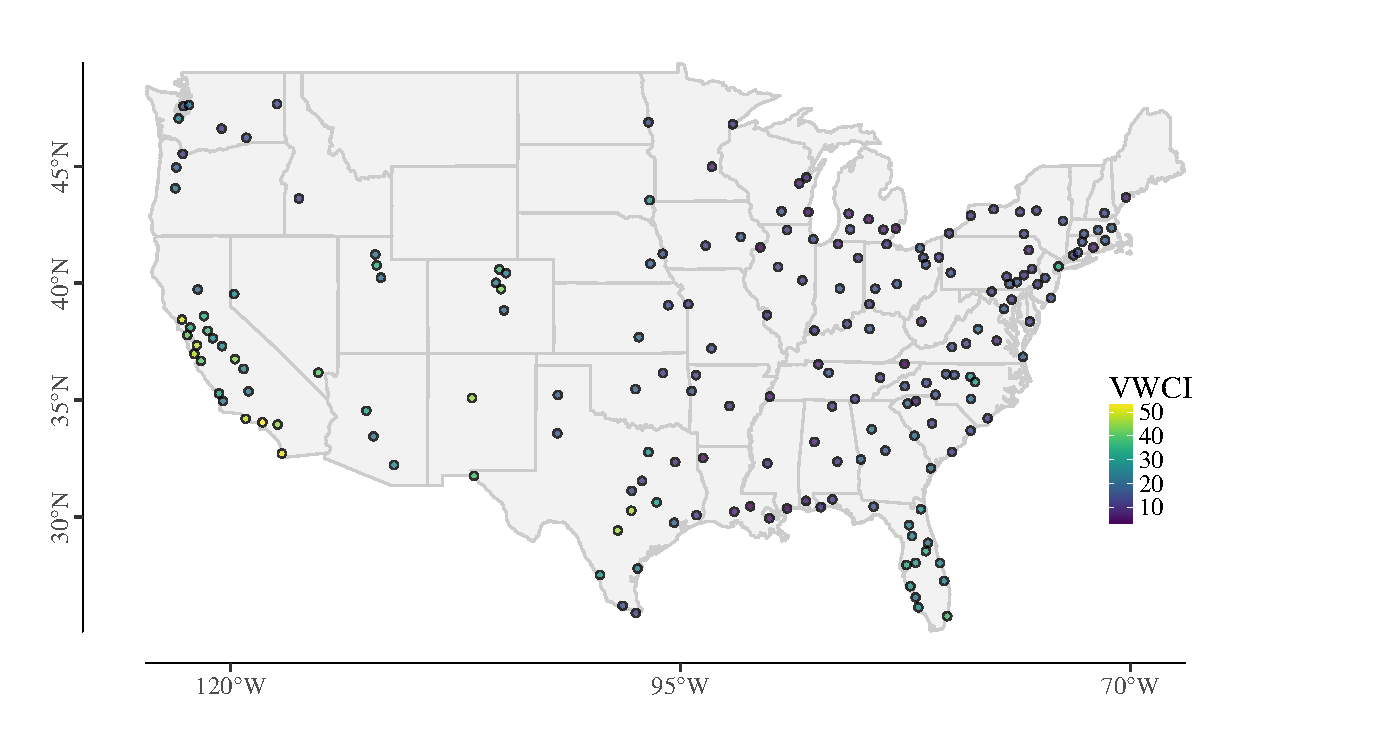
\includegraphics[width=6.5in,angle=0]{figures_si/vwci_map-1} \caption[Map of cities with VWCI scores]{Map of cities with VWCI scores.}\label{fig:vwci_map}
\end{figure}



% jg_tex_chunk_hook

\begin{figure}[H]
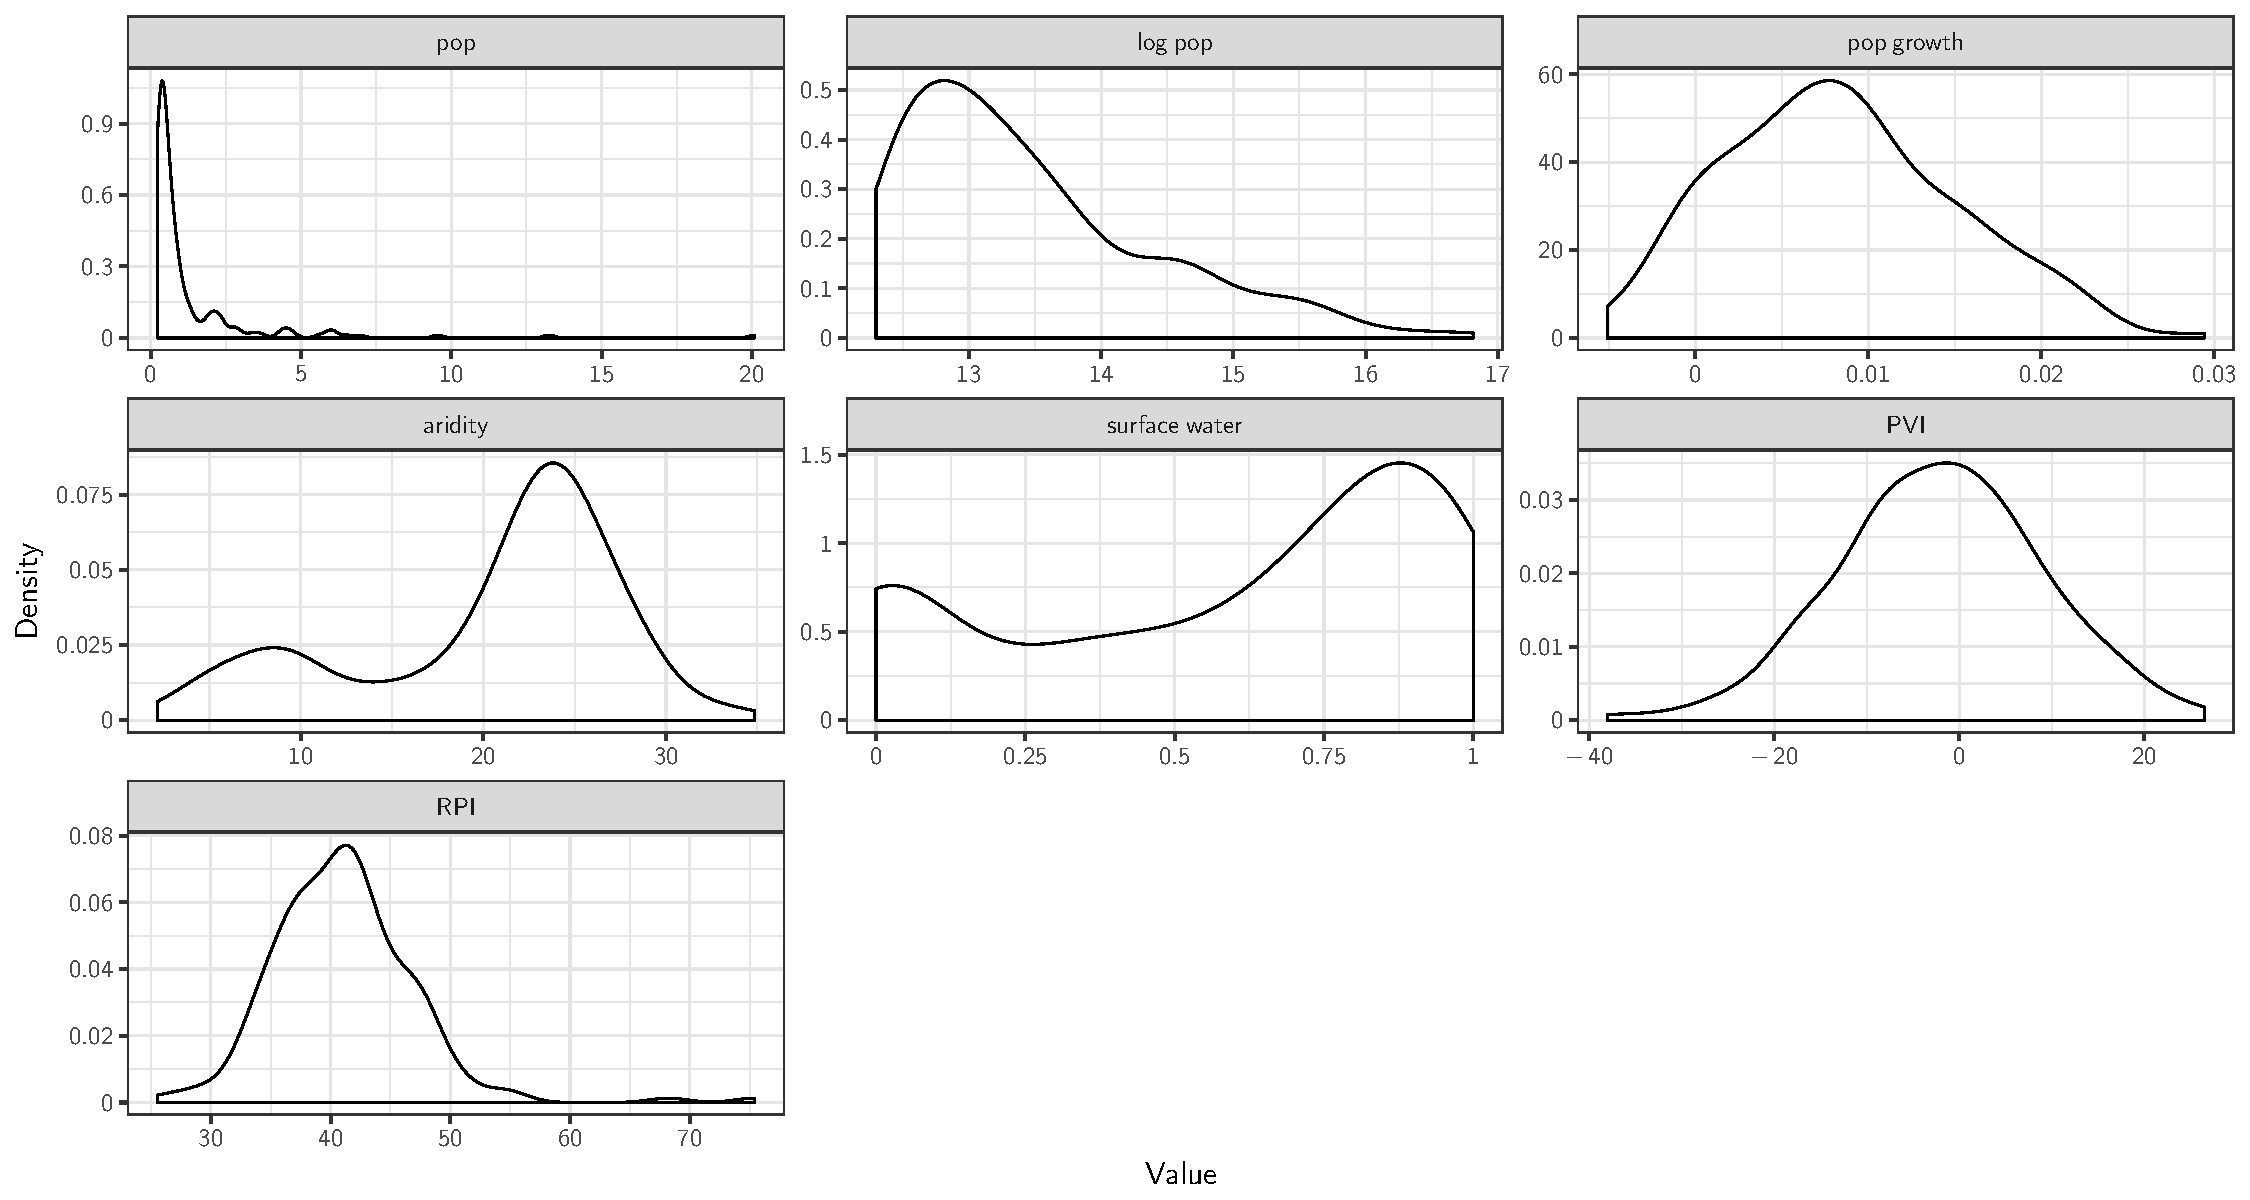
\includegraphics[width=6in]{figures_si/msa_vars_distribution-1} \caption[Kernel-density distribution of MSA-level covariates]{Kernel-density distribution of MSA-level covariates. Population in millions and RPI in thousands of chained 2009 dollars.}\label{fig:msa_vars_distribution}
\end{figure}



% jg_tex_chunk_hook

\begin{figure}
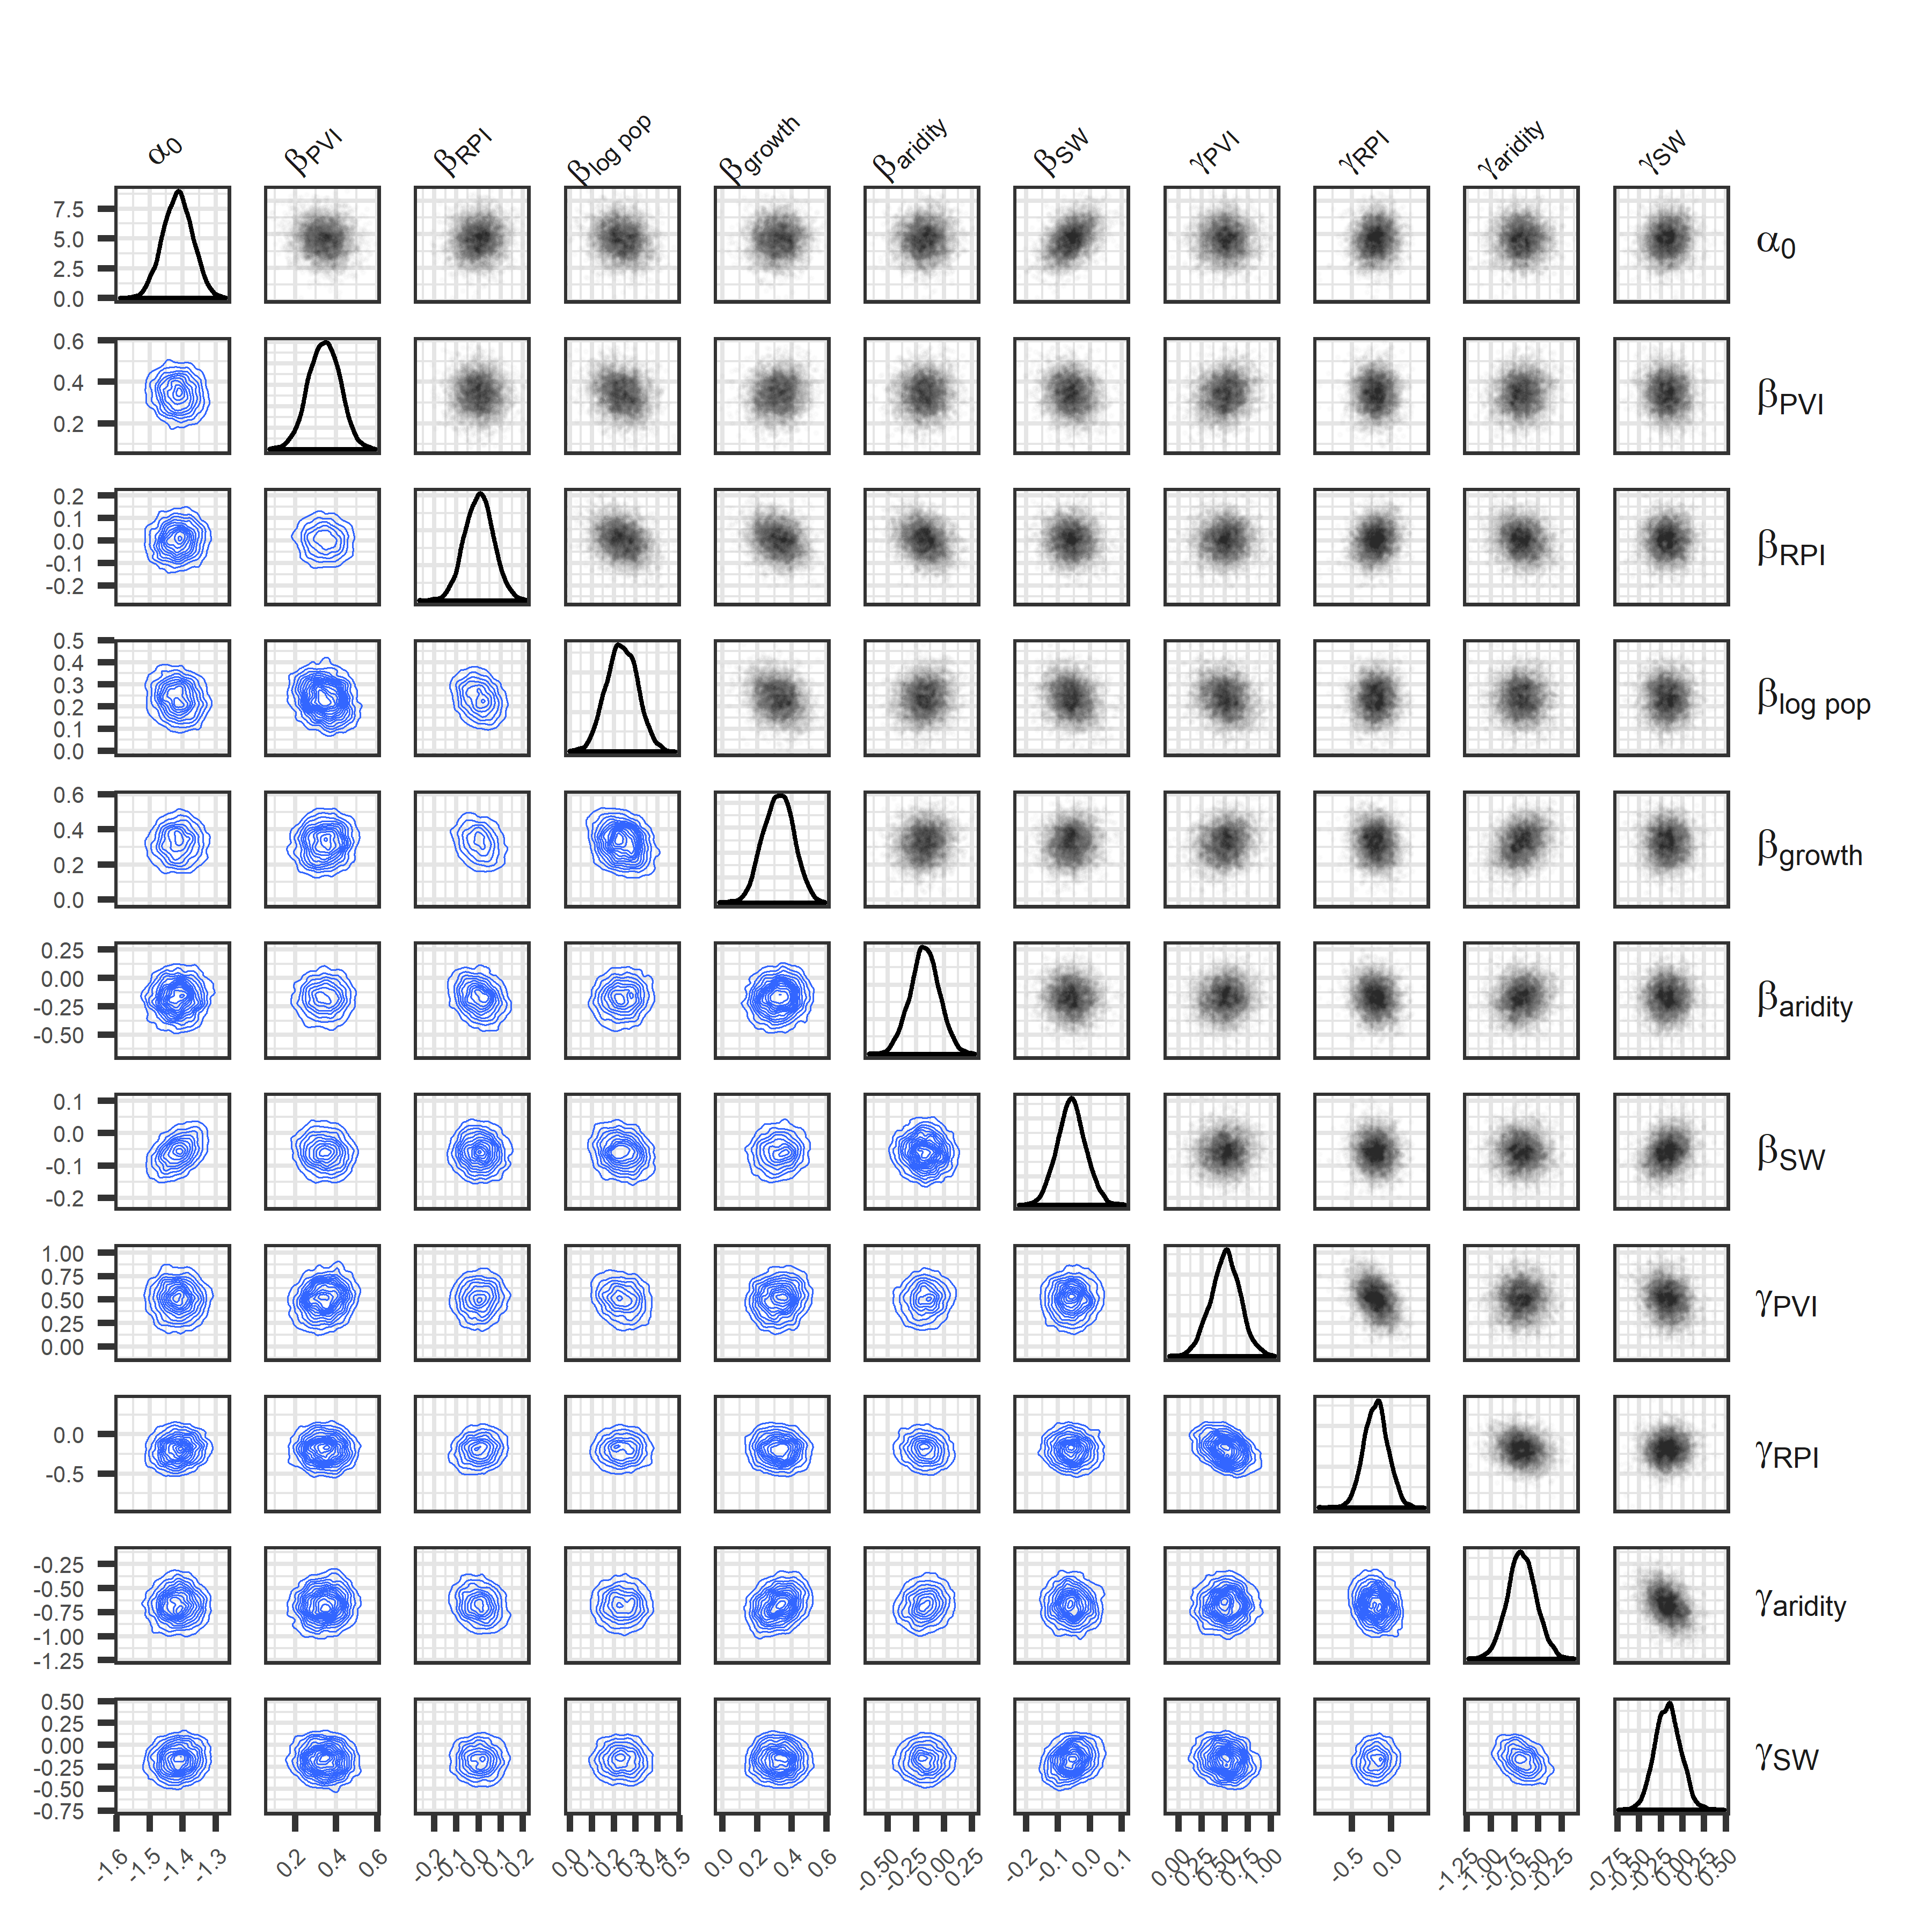
\includegraphics[width=6.25in]{figures_si/vwci_pairs_plot-1} \caption[Correlation plot of posterior probability distribution of regression coefficients $\alpha$, $\beta$, and $\gamma$ for VWCI]{Correlation plot of posterior probability distribution of regression coefficients $\alpha$, $\beta$, and $\gamma$ for VWCI. The diagonal panels show the probability density for each coefficient, panels in the upper triangle show scatterplots of 4000 HMC samples, and panels in the lower triangle show joint probability density contours corresponding to the scatterplot in the upper triangle. Slight correlations are apparent, as between $\gamma_{\text{aridity}}$ and $\gamma_{\text{SW}}$, $\gamma_{\text{PVI}}$ and $\gamma_{\text{RPI}}$, and $\beta_{\text{SW}}$ and $\alpha_0$, but these are small enough not to pose problems apart from slightly increasing the uncertainty in the parameter estimates.}\label{fig:vwci_pairs_plot}
\end{figure}



% jg_tex_chunk_hook

\begin{figure}
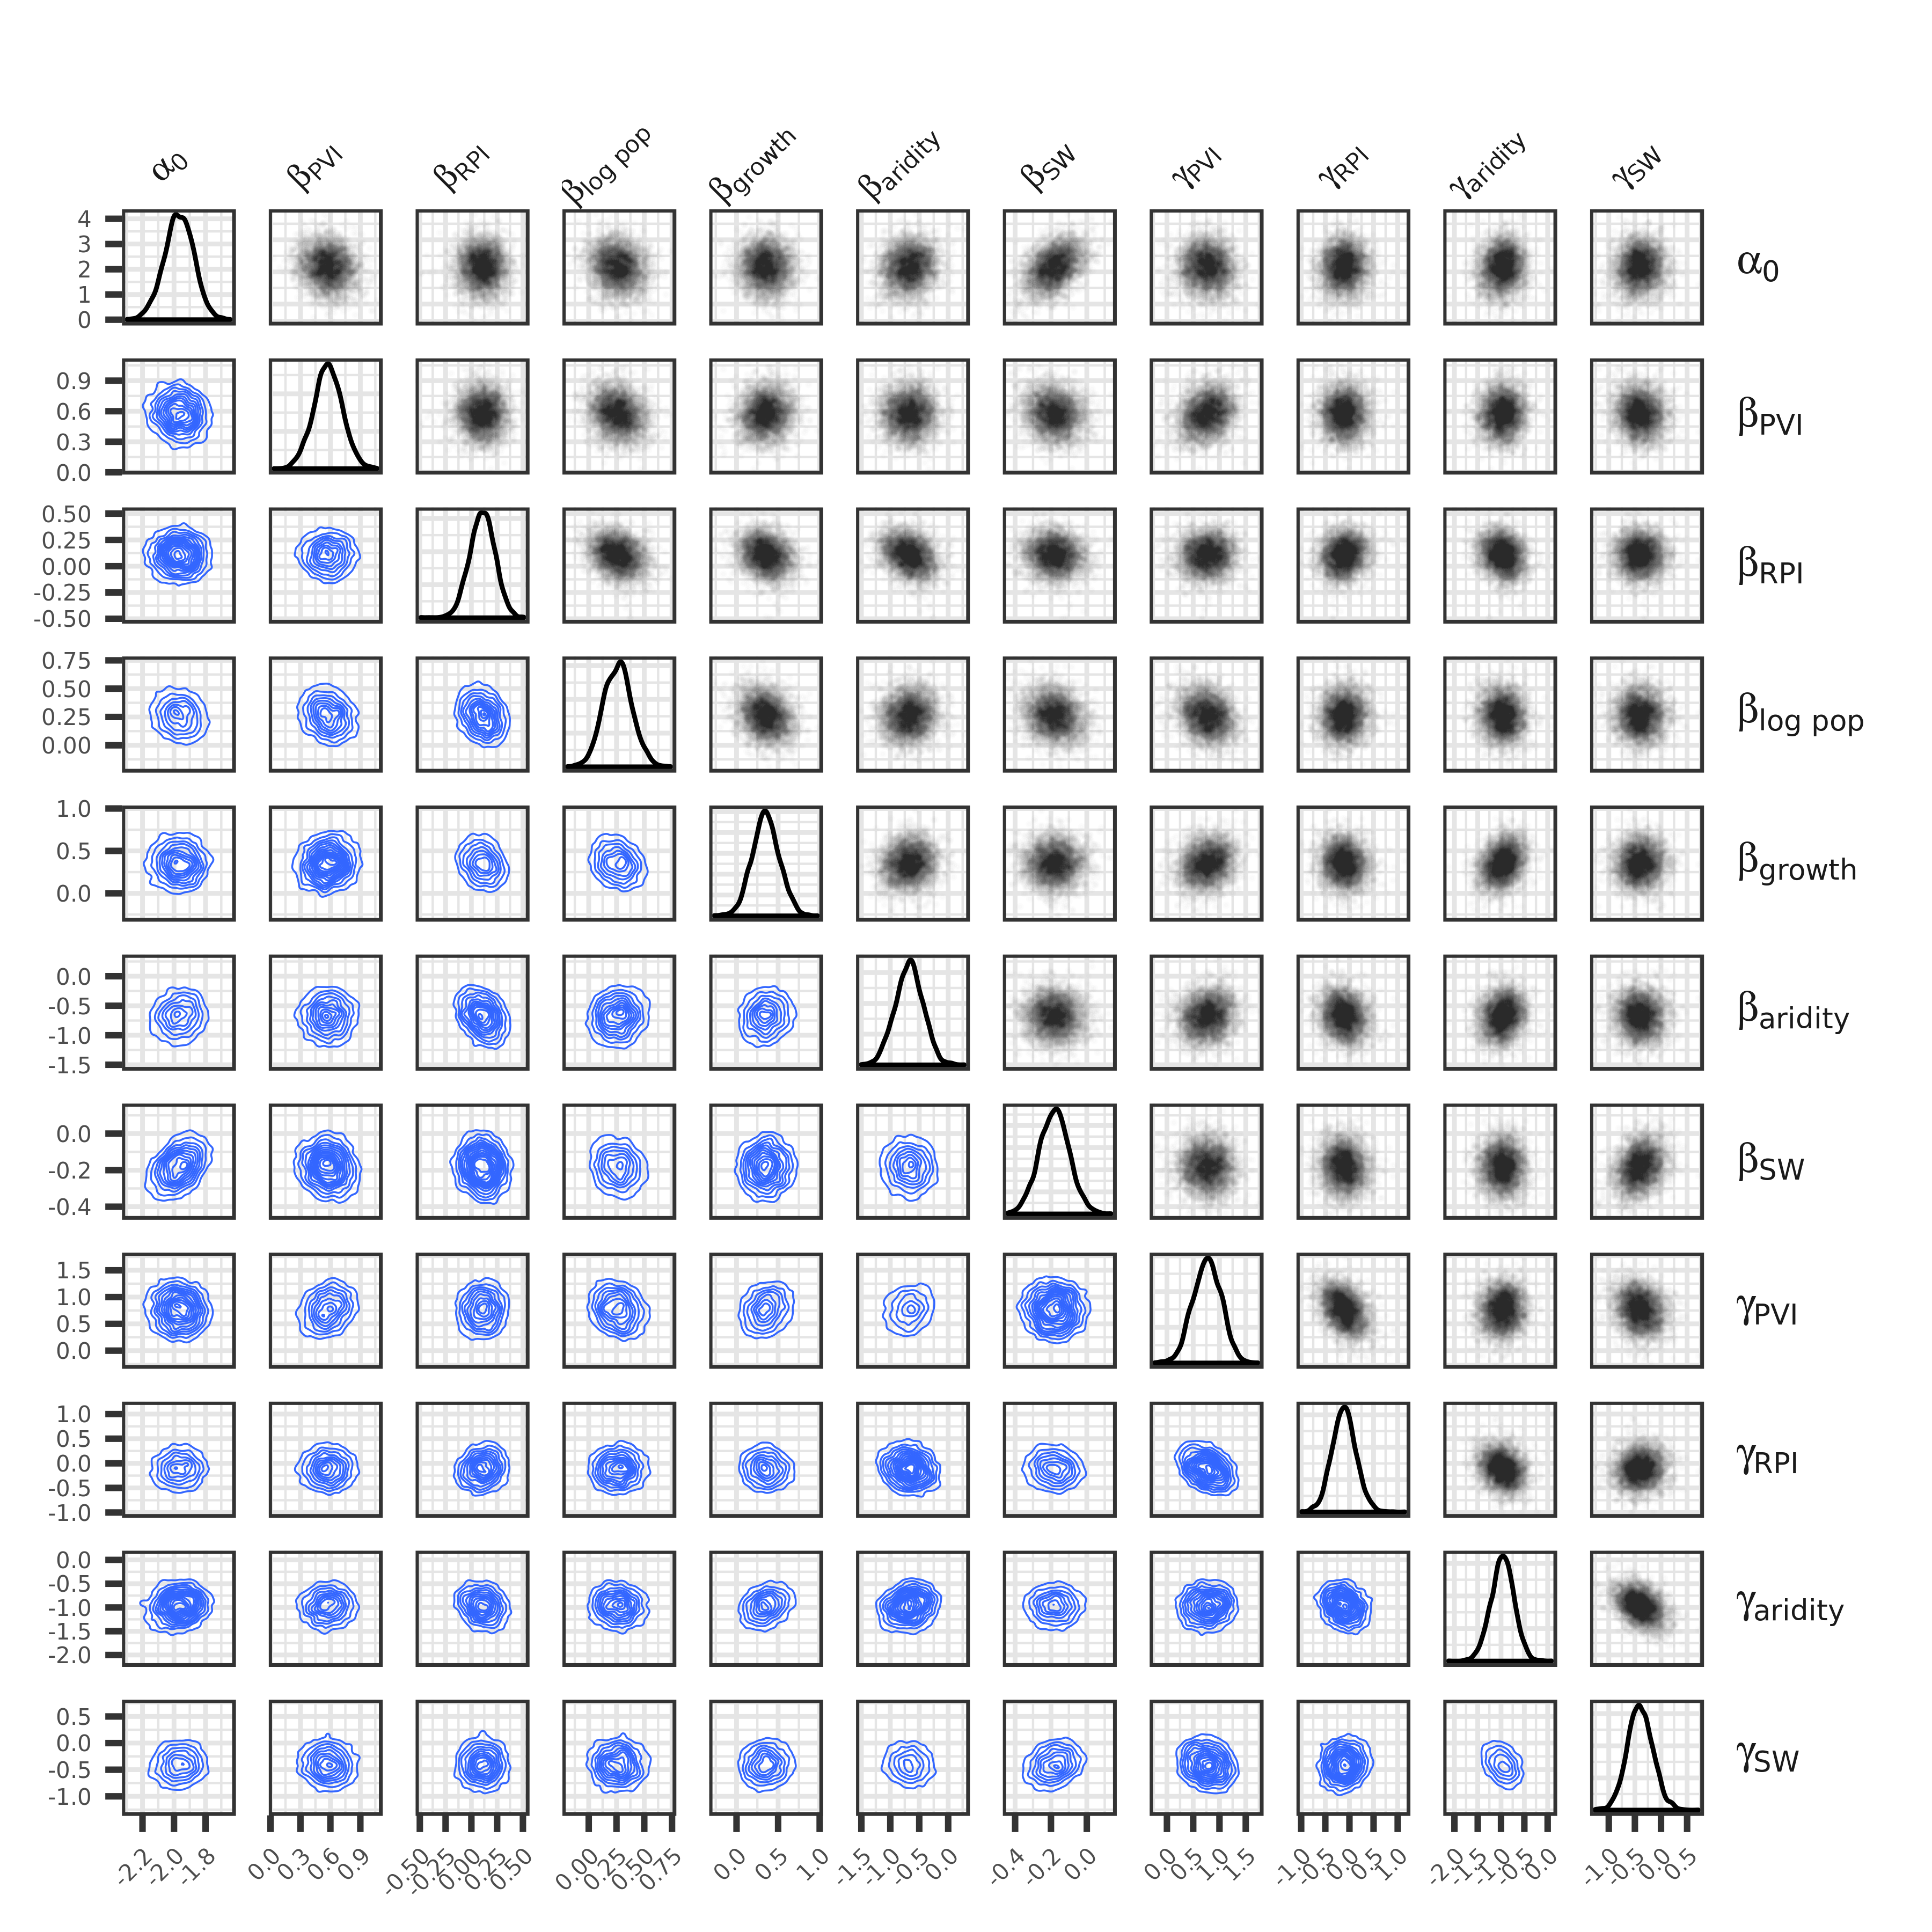
\includegraphics[width=6.25in]{figures_si/req_pairs_plot-1} \caption[Correlation plot of posterior probability distribution of regression coefficients $\alpha$, $\beta$, and $\gamma$ for requirements]{Correlation plot of posterior probability distribution of regression coefficients $\alpha$, $\beta$, and $\gamma$ for requirements.}\label{fig:req_pairs_plot}
\end{figure}



% jg_tex_chunk_hook

\begin{figure}
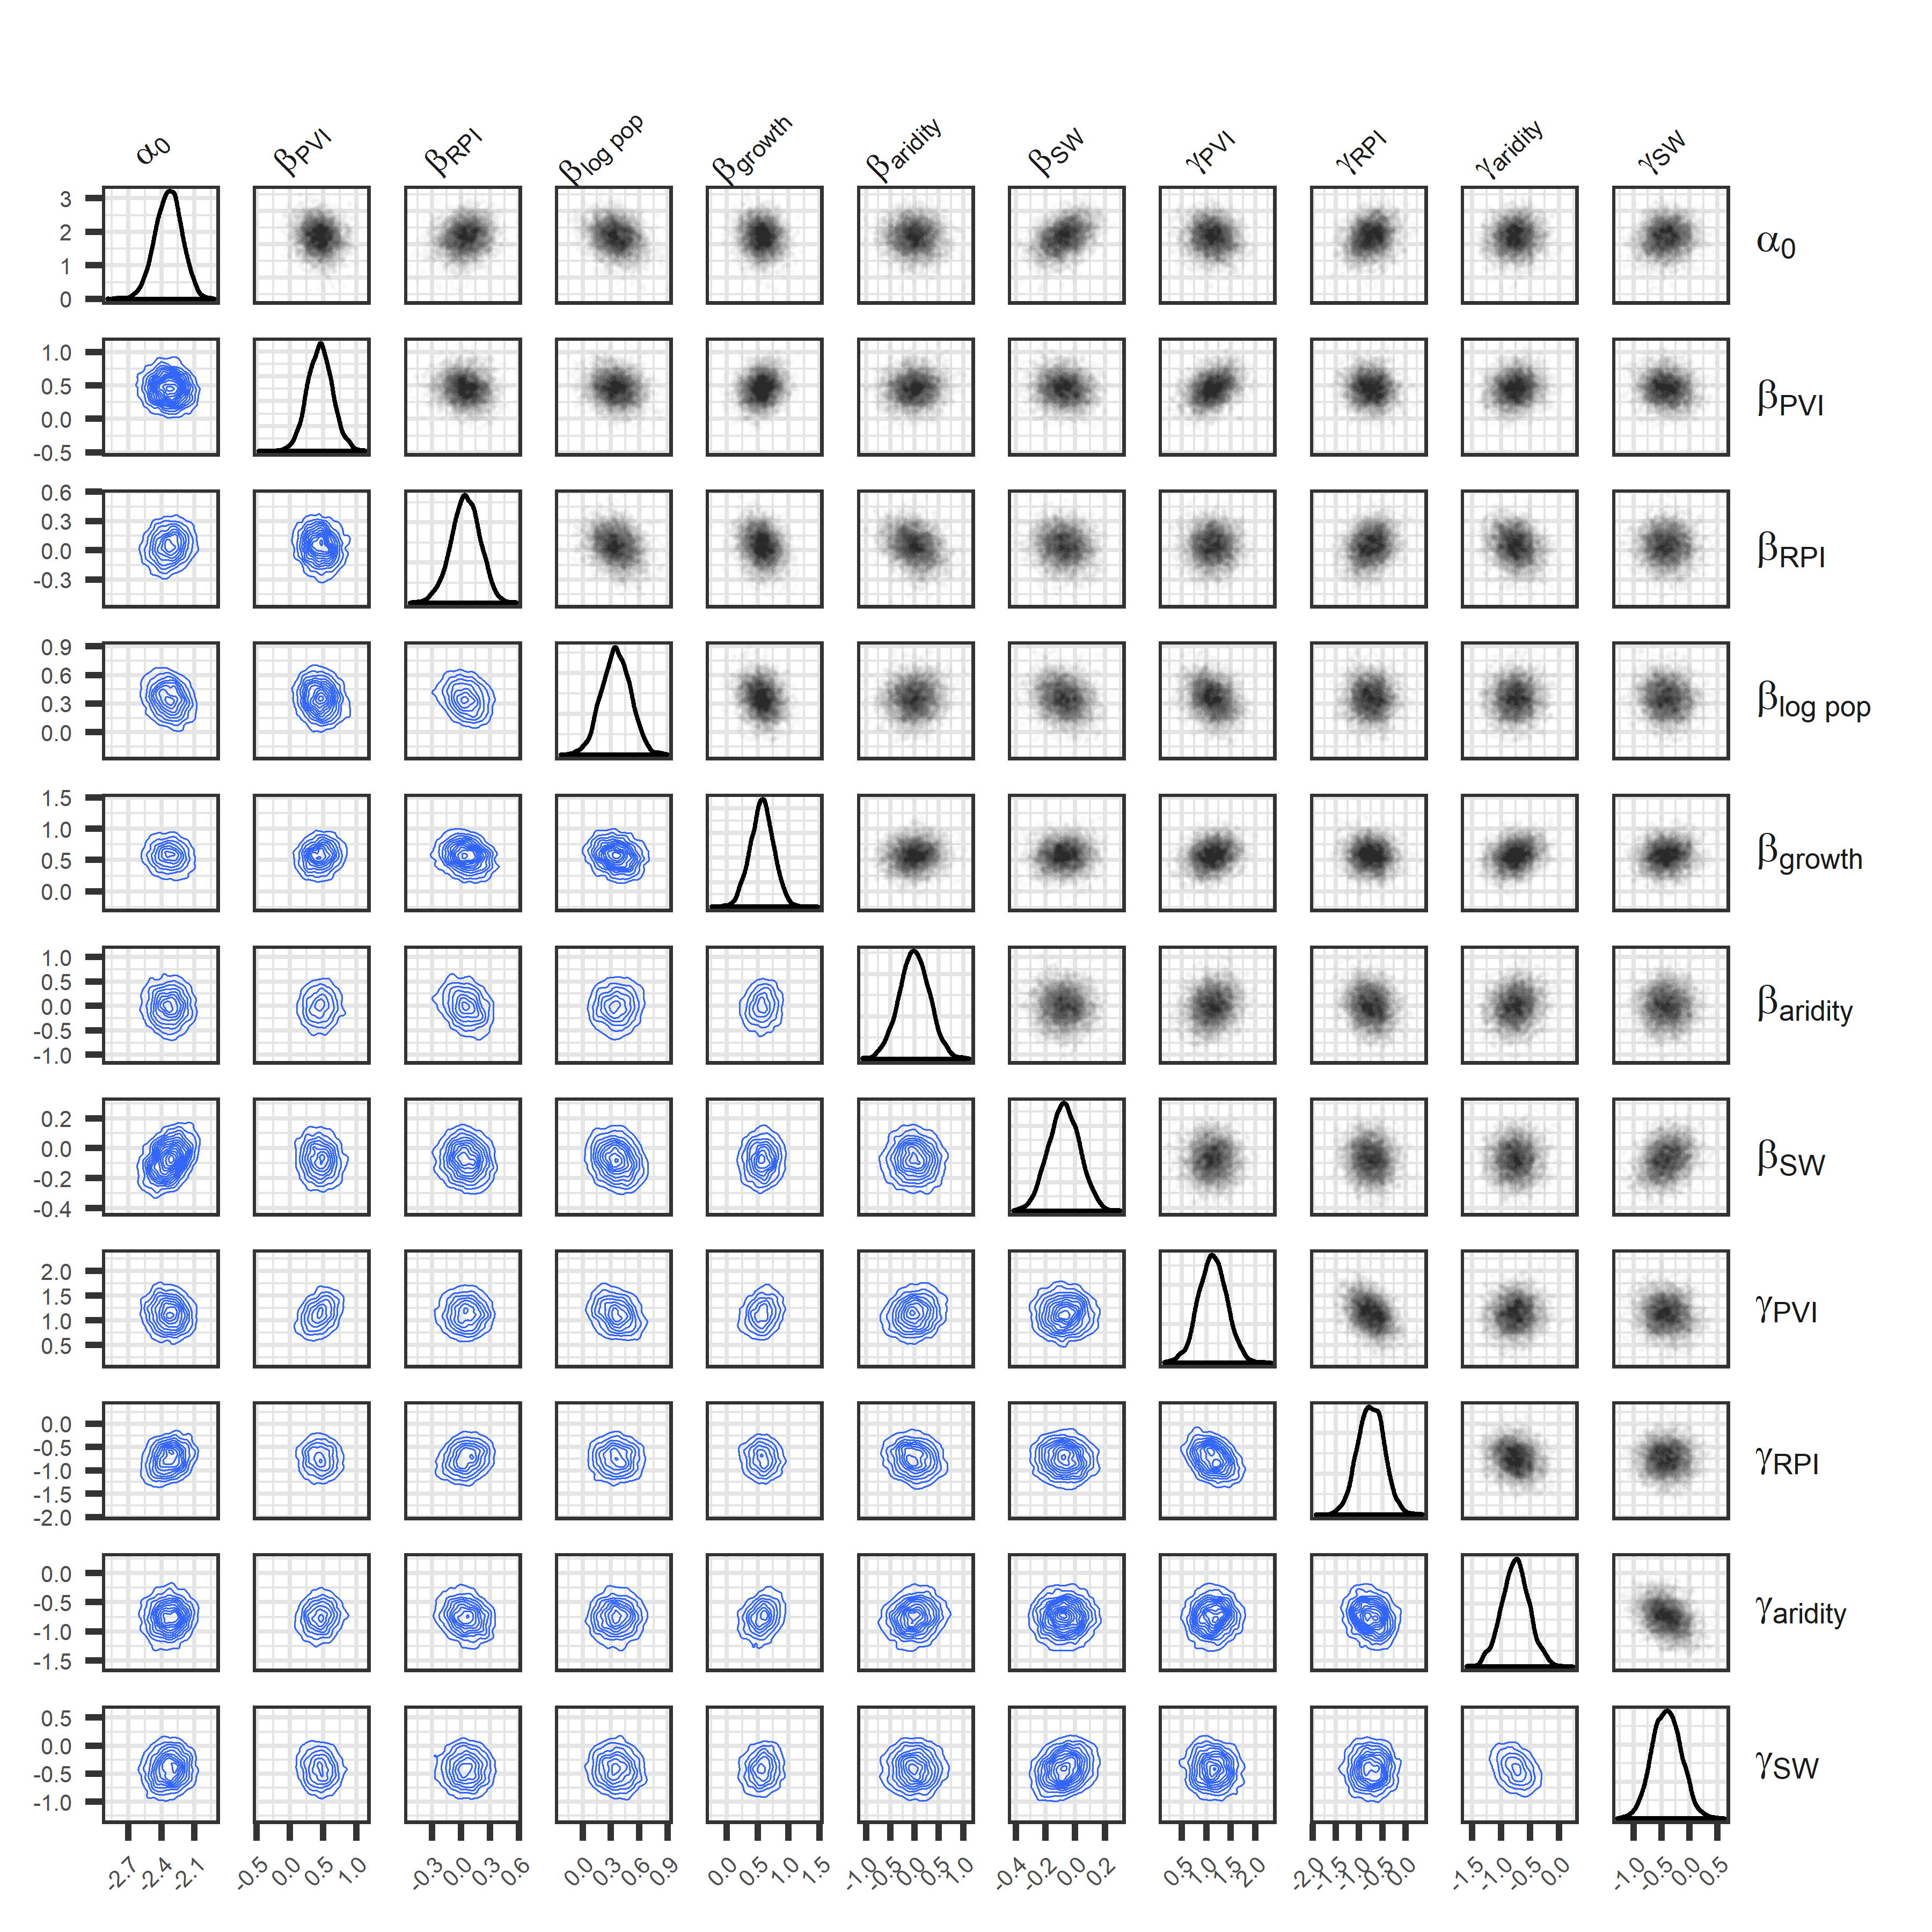
\includegraphics[width=6.25in]{figures_si/reb_pairs_plot-1} \caption[Correlation plot of posterior probability distribution of regression coefficients $\alpha$, $\beta$, and $\gamma$ for rebates]{Correlation plot of posterior probability distribution of regression coefficients $\alpha$, $\beta$, and $\gamma$ for rebates.}\label{fig:reb_pairs_plot}
\end{figure}



\clearpage
\section{Tables S1--S7}
\subsection*{Table S1 Caption}
\begin{table}[H]
\centering
\caption{Conservation scores and covariates for  cities: VWCI = Vanderbilt Water Conservation Index (total \# of conservation measures), Req.\ = \# requirements, Reb.\ = \# rebates, PVI = Cook Partisan Voting Index, Aridity = K\"oppen aridity index, RPI\ = per-capita real personal income (thousands of regionally adjusted chained 2009 dollars), Pop.\ = population (thousands), Growth = population growth rate (2010--2014), Surf.\ W.\ = surface-water fraction.}
\label{tab:vwci}
\end{table}

\subsection*{Table S2 Caption}
\begin{table}[H]
\centering
\caption{State-level covariates: PVI = Cook Partisan Voting Index, RPI = per-capita real personal income (thousands of regionally-adjusted chained 2009 dollars), Aridity = the K\"oppen aridity index, Surf.\ W.\ = the surface-water fraction.}
\label{tab:state}
\end{table}

\subsection*{Table S3}
% latex table generated in R 3.3.3 by xtable 1.8-2 package
% Mon Apr  3 14:54:55 2017
\begin{table}[H]
\centering
\begin{tabular}{rrrrr}
  \hline
Model & LOO-IC & s.e.\ LOO-IC & $\text{ELPD}_{\text{\scshape loo}}$ & s.e.\ $\text{ELPD}_{\text{\scshape loo}}$ \\ 
  \hline
hierarchical beta-binomial & 1249.4 & 20.5 & -624.7 & 10.2 \\ 
  hierarchical binomial & 1334.3 & 44.3 & -667.2 & 22.2 \\ 
  single-level binomial & 2064.6 & 143.8 & -1032.3 & 71.9 \\ 
  single-level beta-binomial & 2438.6 & 183.4 & -1219.3 & 91.7 \\ 
   \hline
\end{tabular}
\caption[Model comparison: LOO.]{Model comparison: LOO = leave-one-out cross-validation, LOO-IC = LOO information criterion, ELPD = expected log pointwise predictive density, and s.e. indicates the standard error of estimates of quantities. Lower values of the information criteria and greater (less negative) values of ELPD indicate superior model performance.} 
\label{tab:loo}
\end{table}

\subsection*{Table S4}
% latex table generated in R 3.3.3 by xtable 1.8-2 package
% Mon Apr  3 14:54:58 2017
\begin{table}[H]
\centering
\begin{tabular}{rrrrr}
  \hline
Model & WAIC & s.e. WAIC & $\text{ELPD}_{\text{\scshape waic}}$ & s.e.\ $\text{ELPD}_{\text{\scshape waic}}$ \\ 
  \hline
hierarchical beta-binomial & 1245.2 & 20.1 & -622.6 & 10.1 \\ 
  hierarchical binomial & 1320.2 & 43.5 & -660.1 & 21.7 \\ 
  single-level binomial & 2063.2 & 143.6 & -1031.6 & 71.8 \\ 
  single-level beta-binomial & 2386.1 & 177.5 & -1193.1 & 88.8 \\ 
   \hline
\end{tabular}
\caption[Model comparison: WAIC]{Model comparison: WAIC = widely applicable information criterion (also known as the Watanabe-Aikake Information Criterion), ELPD = expected log-probability density, and s.e. indicates the standard error of estimates of quantities. Lower values of the information criteria and greater (less negative) values of ELPD indicate superior model performance.} 
\label{tab:waic}
\end{table}

\subsection*{Table S5 Caption}
\begin{table}[H]
\centering
\caption{Posterior probability distributions of regression coefficients for VWCI: mean, standard error of the mean, standard deviation of the posterior, quantiles of the posterior, and the Gelman-Rubin potential scale-reduction factor $\hat R$. $\gamma$ coefficients correspond to state-level effects, $\beta$ coefficients to MSA-level effects, $\delta$ coefficients represent state-level intercepts, $\alpha_0$ is the overall intercept, and $\phi$ characterizes the overdispersion of the beta-binomial distribution. For more detail, see Materials and Methods.}
\label{tab:vwci_posterior}
\end{table}


\subsection*{Table S6 Caption}
\begin{table}[H]
\centering
\caption{Posterior probability distribution of regression coefficients for requirements}
\label{tab:req_posterior}
\end{table}


\subsection*{Table S7 Caption}
\begin{table}[H]
\centering
\caption{Posterior probability distribution of regression coefficients for rebates}
\label{tab:reb_posterior}
\end{table}



\section*{Captions for Datasets S1--S2}

\subsection*{Dataset S1: MSA-Level Data}

This dataset contains MSA-level data: the FIPS (Federal Information Processing Standard) code for the MSA,
the name of the MSA, the central city, state, latitude, longitude,
VWCI, number of water-conservation requirements, number of rebate policies for water-conservation actions,
the average annual precipitation (in millimeters) temperature (in Celsius), and K\"oppen aridity index, for the central city,
the Cook Partisan Voting Index for the counties of the MSA,
the 2014~population and average annual population growth rate from 2010--2014 for the MSA,
the fraction of the municipal water supply derived from surface water,
the BEA 2014 regional price parity and per-capita real personal income for the MSA (in chained regionally-adjusted 2009 dollars).

\subsection*{Dataset S2: State-Level Data}

This dataset contains stae-level data: the FIPS code for the state, the abbreviation and name of the state,
the average annual precipitation (in millimeters), temperature (in Celsius), and K\"oppen aridity index for the state,
the state-level Cook Partisan Voting Index,
the fraction of the state water supply derived from surface water,
and the BEA 2014 state-level regional price parity and per-capita real personal income (in chained regionally-adjusted 2009 dollars).

\section*{Data Analysis Scripts S1}

The zip file \verb+scripts_S1.zip+ contains R and Stan scripts to reproduce the regression analysis presented here.
To reproduce the analysis, unzip the file with the scripts, copy Datasets S1 and S2 into the \verb+data+ subdirectory, and run the script \verb+gilligan_vwci_ef_2017.R+ in R.

This paper was produced with the following R packages:

% jg_tex_chunk_hook

\begin{verbatim}
## R version 3.3.3 (2017-03-06)
## Platform: x86_64-pc-linux-gnu (64-bit)
## Running under: Ubuntu 16.04.2 LTS
## 
## locale:
##  [1] LC_CTYPE=en_US.UTF-8       LC_NUMERIC=C              
##  [3] LC_TIME=en_US.UTF-8        LC_COLLATE=en_US.UTF-8    
##  [5] LC_MONETARY=en_US.UTF-8    LC_MESSAGES=en_US.UTF-8   
##  [7] LC_PAPER=en_US.UTF-8       LC_NAME=C                 
##  [9] LC_ADDRESS=C               LC_TELEPHONE=C            
## [11] LC_MEASUREMENT=en_US.UTF-8 LC_IDENTIFICATION=C       
## 
## attached base packages:
## [1] stats     graphics  grDevices utils     datasets  methods   base     
## 
## other attached packages:
##  [1] jgally_1.2.9.9999    jgmcmc_1.1           loo_1.1.0           
##  [4] rstan_2.14.2         StanHeaders_2.14.0-1 viridis_0.4.0       
##  [7] viridisLite_0.2.0    ggthemes_3.4.0       xtable_1.8-2        
## [10] gridExtra_2.2.1      ggrepel_0.6.5        extrafont_0.17      
## [13] stringr_1.2.0        readxl_0.1.1         dplyr_0.5.0         
## [16] purrr_0.2.2          readr_1.1.0          tidyr_0.6.1         
## [19] tibble_1.3.0         ggplot2_2.2.1        tidyverse_1.1.1     
## [22] pacman_0.4.1         knitr_1.15.1        
## 
## loaded via a namespace (and not attached):
##  [1] reshape2_1.4.2     haven_1.0.0        lattice_0.20-34   
##  [4] colorspace_1.3-2   stats4_3.3.3       foreign_0.8-67    
##  [7] DBI_0.6-1          RColorBrewer_1.1-2 modelr_0.1.0      
## [10] matrixStats_0.51.0 plyr_1.8.4         munsell_0.4.3     
## [13] gtable_0.2.0       rvest_0.3.2        psych_1.7.3.21    
## [16] evaluate_0.10      inline_0.3.14      GGally_1.3.0      
## [19] forcats_0.2.0      parallel_3.3.3     Rttf2pt1_1.3.4    
## [22] broom_0.4.2        Rcpp_0.12.10       scales_0.4.1      
## [25] jsonlite_1.3       mnormt_1.5-5       digest_0.6.12     
## [28] hms_0.3            stringi_1.1.3      grid_3.3.3        
## [31] tools_3.3.3        magrittr_1.5       lazyeval_0.2.0    
## [34] extrafontdb_1.0    xml2_1.1.1         lubridate_1.6.0   
## [37] assertthat_0.1     reshape_0.8.6      httr_1.2.1        
## [40] R6_2.2.0           nlme_3.1-131
\end{verbatim}



%
% BEGIN LARGE TABLE SECTION
%
\iffalse
%
\section*{Captions for Large Tables S1, S2, S5--S7}
\subsection*{Table S1 Caption}
\setcounter{table}{0}%
\begin{table}[H]
\centering
\caption{Conservation scores and covariates for  cities: VWCI = Vanderbilt Water Conservation Index (total \# of conservation measures), Req.\ = \# requirements, Reb.\ = \# rebates, PVI = Cook Partisan Voting Index, Aridity = K\"oppen aridity index, RPI\ = per-capita real personal income (thousands of regionally adjusted chained 2009 dollars), Pop.\ = population (thousands), Growth = population growth rate (2010--2014), Surf.\ W.\ = surface-water fraction.}
\end{table}


\subsection*{Table S2 Caption}
\setcounter{table}{1}%
\begin{table}[H]
\centering
\caption{State-level covariates: PVI = Cook Partisan Voting Index, RPI = per-capita real personal income (thousands of regionally-adjusted chained 2009 dollars), Aridity = the K\"oppen aridity index, Surf.\ W.\ = the surface-water fraction.}
\end{table}


\subsection*{Table S5 Caption}
\setcounter{table}{4}%
\begin{table}[H]
\centering
\caption{Posterior probability distributions of regression coefficients for VWCI: mean, standard error of the mean, standard deviation of the posterior, quantiles of the posterior, and the Gelman-Rubin potential scale-reduction factor $\hat R$. $\gamma$ coefficients correspond to state-level effects, $\beta$ coefficients to MSA-level effects, $\delta$ coefficients represent state-level intercepts, $\alpha_0$ is the overall intercept, and $\phi$ characterizes the overdispersion of the beta-binomial distribution. For more detail, see Materials and Methods.}
\end{table}


\subsection*{Table S6 Caption}
\setcounter{table}{5}%
\begin{table}[H]
\centering
\caption{Posterior probability distribution of regression coefficients for requirements}
\end{table}


\subsection*{Table S7 Caption}
\setcounter{table}{6}%
\begin{table}[H]
\centering
\caption{Posterior probability distribution of regression coefficients for rebates}
\end{table}

%
\fi
%
% END LARGE TABLE SECTION
%
% Bibliography
% \bibliography{gilligan_vwci_ef_2017}

\end{document}



